\section{Centrality}

Consider the following graphs, which nodes are central?

\begin{figure}[H]
	\centering
	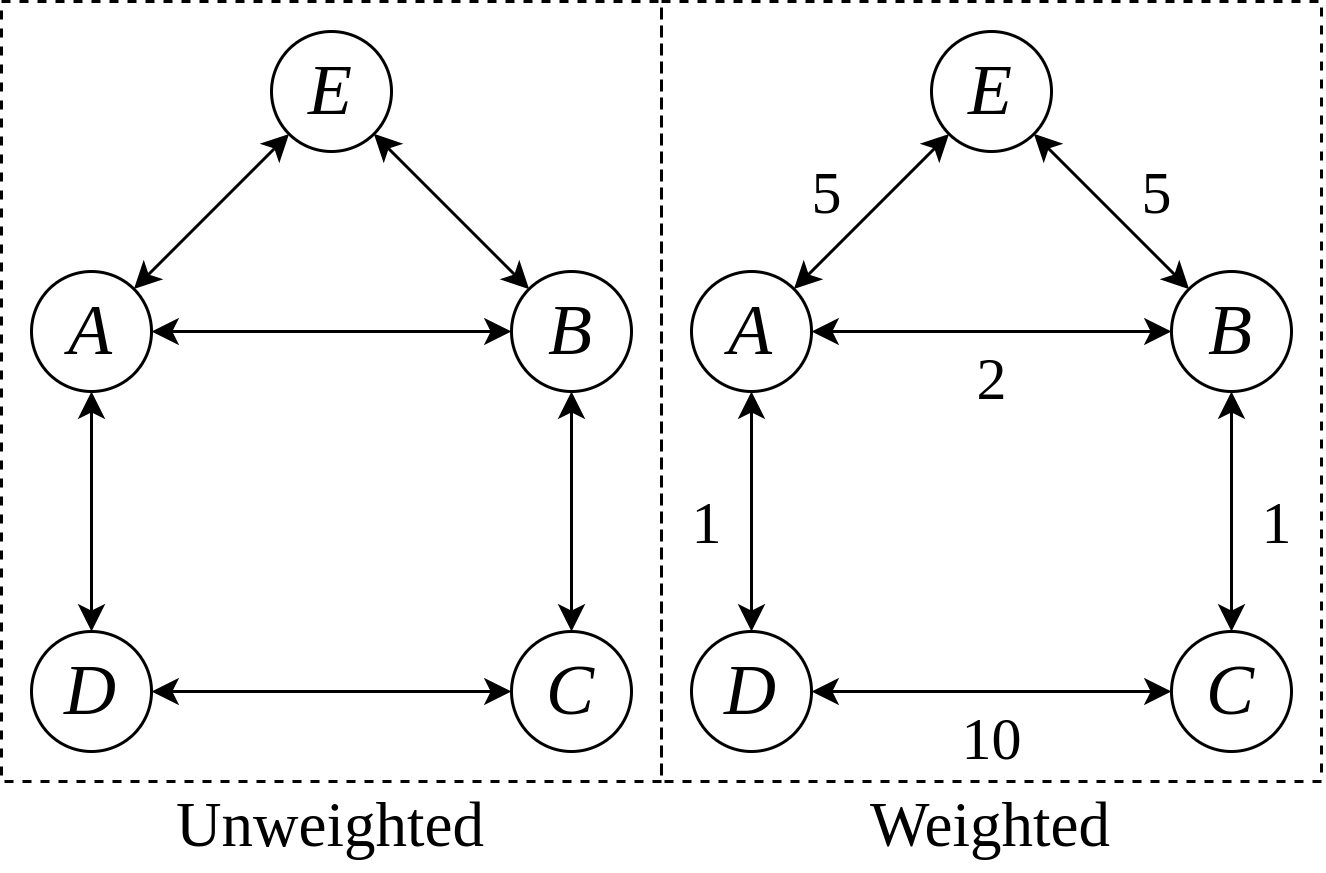
\includegraphics[width = .5\linewidth]{figs/simple_graph.png}
	\caption{Simple example undirected graph unweighted and weighted isomorphs (from \cite{Stephenson_1989})}
	\label{fig:simple_graph}
\end{figure}

From Figure \ref{fig:simple_graph} it is apparent that $A$ and $B$ are more central than the other nodes. Graphs, however, need not have a geometric center nor any plainly obvious 2-D geometry. Take, for example, a network of communications satellites in low Earth orbit. Although the state of the network could, at any point, be projected onto a 2-D surface it would be arbitrary where the corners of the map should be located. In 3-D space all satellites would be approximately the same distance from the geometric center, the center of the Earth, a location where there will be no proximate satellites. Centrality, thus, must have a more abstract definition. There are four commonly used metrics for centrality, degree centrality, closeness centrality, betweenness centrality, and information centrality. These will be defined in the below subsections.

\subsection{Degree Centrality}

A computationally simple way to compute adjacency-focused centrality is degree centrality. Degree centrality is defined as

\begin{equation}
	\Omega_d(v) = \frac{\eta(v)}{n - 1}
\end{equation}

where $\eta(v)$ is a function returning a value computed from the adjacency of node $v$. Degree is the number of adjacent nodes adjacent to a given node. A cell tower has high degree centrality as part of the cellular communications network.

\subsection{Closeness Centrality}

For a graph $G$, the sets of shortest paths from each node $v$ to all other nodes $R_{v,U}$ and vice versa $R_{U,v}$ are known. Closeness centrality is defined as

\begin{equation}
	\Omega_c(v) = \frac{n - 1}{\sum_{u \in U} \eta(v, u)}
\end{equation}

where $n$ is the cardinality of $V$ and $\eta(v, u)$ is the cost of the shortest path from $v$ to $u$. Closeness centrality reflects how close a given node is to those nodes reachable from it via shortest paths. St. Louis has high closeness centrality as part of the US freeway system.

\subsection{Betweenness Centrality}

For a graph $G$, the sets of shortest paths from each node $v$ to all other nodes $R_{v,U}$ and vice versa $R_{U,v}$ are known. Betweenness centrality is defined as

\begin{equation}
	\Omega_b(v) = \sum_{o, d \in V}\frac{\sigma(o, d\ |\ v)}{\sigma(o, d)}\label{eq:betweenness_centrality}
\end{equation}

where $\sigma(o, d\ |\ v)$ is the weighted sum of the set of shortest paths between $o$ and $d$ which contain $v$ and $\sigma(o, d)$ is the weighted sum of the set of shortest paths between $o$ and $d$. Betweenness centrality reflects the relative volume of use for a node in a graph (and may also be computed for edges). The Denver airport has high betweenness centrality as part of the US domestic aviation network.

\subsection{Information Centrality}

Conceptually the information content of a node on a graph is the path information gained after leaving that node. There may be many paths on a graph which pass through a given node and thus an expectation must be computed. The following derivation is based on \cite{Stephenson_1989} which is the original publication on information centrality.

For each O/D pair in $o,d \in V$ there is a set of paths $P_{od} = \{P_{od}(1),P_{od}(2), \dots, P_{od}(n_{od})\}$ with associated costs $C_{od}$. Picking $o=A$ and $d=B$ from the graph in Figure \ref{fig:simple_graph}, $P_{AB}$ contains $P_{AB}(1) = A - B$, $P_{AB}(2) = A - E - B$, and $P_{AB}(3) = A - D - C - B$. The costs of the paths will be $C_{AB}(1) = 1$, $C_{AB}(2) = 2$, and $C_{AB}(3) = 3$ for the unweighted graph and $C_{AB}(1) = 2$, $C_{AB}(2) = 10$, and $C_{AB}(3) = 12$ for the weighted graph. Under the assumption that lower-cost paths are more likely to be taken and knowing that information is inversely proportional to probability it should be apparent that the information content of the indirect paths is greater than that of the direct path. It should also be apparent that the edge weights increase the information disparity. Consider $I_{od}(i) = C_{od}(i)^{-1}$ as an analogue for information content (this is used rather than \eqref{eq:information_content} for computational simplicity). Entropy for node $o$ with respect to node $d$ can thus be computed as

\begin{equation}
	S_{od} = \sum_{i = 1}^{n_{od}}W_{od}(i)C_{od}(i)
\end{equation}

where

\begin{equation}
	W_{od}(i) = \frac{I_{od}(i)}{\sum_{i = 1}^{n_{od}} I_{od}(i)}
\end{equation}

Generalizing path entropy to node entropy means considering how node $o$ interacts with all possible O/D pairs which. For the sake of computational efficiency, this generalization can be formulated into a matrix-operations based process as in \cite{Stephenson_1989}. Information centrality for the nodes in $G = \{V, E\}$ is based on the inverse incidence matrix $B$ whose elements are

\begin{align}
	b_{ij} = \begin{cases}
		1 & (i, j) \not\in E \\
		1 - \eta(i, j) & otherwise
	\end{cases}\\
	b_{ii} = 1 + \sum_{(i, j) \in E_i} \eta(i, j)
\end{align}

where $\eta(i, j)$ is a function returning edge costs. The diagonal elements of $B$ are the degrees of $V$ plus self-connection and the non-diagonal elements are 1 if no direct connection exists and less than 1 where one does exist. Rows and columns of $B$ all have the same sum if $G$ is reciprocal. The information for each node can be computed form the incidence matrix $C = D^{-1}$ as

\begin{equation}
	\Omega_i(v) = \frac{n}{nc_{vv} + \sum_{u = 1}^{n} c_{uu} - 2 \sum_{u = 1}^{n}c_{vu}}\label{eq:information_centrality}
\end{equation}

Information centrality for a node should be interpreted as being, roughly, the degree to which that node is determinative of future nodes on a path between an unknown origin and destination. A node with high information content is a node which both appears on many lowest-cost paths and one which, generally, limits the set of paths after it. As an example, the phrase "medium-rare" may be preceded by many words but will usually be followed by a type of red meat. Information centrality should be thought of as the opposite of network entropy.

\subsection{Comparison}

The methods of computing centrality are compared for the simple graph shown in Figure \ref{fig:simple_graph}.

\begin{table}[H]
	\centering
	\caption{Centrality for simple undirected and unweighted example graph}
	\label{tab:unweighted_centrality}
	\begin{tabular}{|C{.2\linewidth}|C{.2\linewidth}|C{.2\linewidth}|C{.2\linewidth}|C{.2\linewidth}|}
		\hline Node & Degree Centrality & Betweenness Centrality & Closeness Centrality & Information Centrality \\
		\hline A & 0.75 & 0.25 & 0.8 & 0.355 \\
		\hline B & 0.75 & 0.25 & 0.8 & 0.355 \\
		\hline C & 0.5 & 0.083 & 0.667 & 0.282 \\
		\hline D & 0.5 & 0.083 & 0.667 & 0.282 \\
		\hline E & 0.5 & 0 & 0.667 & 0.275 \\
		\hline
	\end{tabular}
\end{table}

\begin{table}[H]
	\centering
	\caption{Centrality for simple undirected and weighted example graph}
	\label{tab:weighted_centrality}
	\begin{tabular}{|C{.2\linewidth}|C{.2\linewidth}|C{.2\linewidth}|C{.2\linewidth}|C{.2\linewidth}|}
		\hline Node & Degree Centrality & Betweenness Centrality & Closeness Centrality & Information Centrality \\
		\hline A & 0.75 & 0.5 & 0.364 & 0.667 \\
		\hline B & 0.75 & 0.5 & 0.364 & 0.667 \\
		\hline C & 0.5 & 0 & 0.286 & 0.535 \\
		\hline D & 0.5 & 0 & 0.286 & 0.535 \\
		\hline E & 0.5 & 0 & 0.182 & 0.646 \\
		\hline
	\end{tabular}
\end{table}

Concerning the isomorphs in Figure \ref{fig:simple_graph}, intuition would say that nodes $A$ and $B$ are most central and this is supported by all centrality measures presented. The principle effects of considering edge weights are that the shortest paths between $C$ and $D$ no longer utilize $(C, D)$, all shortest paths include $A$ or $B$, and 3 include $(A, B)$. The differences are not attested to by degree centrality which is identical among isomorphs. The increased reliance of the network on $A$ and $B$ is reflected in the remaining centrality metrics. The lower diversity of paths for the weighted graph is reflected in lower nodal information content.

